% !TeX document-id = {c68f4be8-c497-43e0-82df-e9ebfbea9577}
% !TeX TXS-program:pdflatex = pdflatex -synctex=1 -interaction=nonstopmode --shell-escape %.tex
% новая команда \RNumb для вывода римских цифр
\documentclass[a4paper,14pt]{article}
\usepackage{amssymb}
\usepackage{amsmath}
\usepackage{amsthm}
\usepackage{caption}
\usepackage{misccorr}
\usepackage[noadjust]{cite}
\usepackage{cmap}
\usepackage[utf8x]{inputenc}
\usepackage[T2A]{fontenc}
\usepackage[english, russian]{babel}
\usepackage{graphics}
\usepackage{graphicx}
\usepackage{textcomp}
\usepackage{verbatim}
\usepackage{makeidx}
\usepackage{geometry}
\usepackage{float}
\usepackage{bm}
\usepackage{esint}
\usepackage{mathtools}
\usepackage{graphicx}
\usepackage{listings}
\usepackage{courier}
\usepackage{multirow}
\usepackage{graphicx}
\usepackage{xcolor}
\usepackage{ucs}
\usepackage{titlesec}

\graphicspath{ {./img/} }

\lstdefinestyle{C}{
	backgroundcolor=\color{white},   % choose the background color
	basicstyle=\footnotesize,        % the size of the fonts that are used for the code
	breakatwhitespace=false,         % sets if automatic breaks should only happen at whitespace
	breaklines=true,                 % sets automatic line breaking
	captionpos=b,                    % sets the caption-position to bottom
	commentstyle=\color{mygreen},    % comment style
	deletekeywords={...},            % if you want to delete keywords from the given language
	escapeinside={\%*}{*)},          % if you want to add LaTeX within your code
	extendedchars=true,              % lets you use non-ASCII characters; for 8-bits encodings only, does not work with UTF-8
	firstnumber=1,                % start line enumeration with line 1000
	frame=single,                    % adds a frame around the code
	keepspaces=true,                 % keeps spaces in text, useful for keeping indentation of code (possibly needs columns=flexible)
	keywordstyle=\color{blue},       % keyword style
	language=C,                 % the language of the code
	morekeywords={*,...},            % if you want to add more keywords to the set
	numbers=left,                    % where to put the line-numbers; possible values are (none, left, right)
	numbersep=5pt,                   % how far the line-numbers are from the code
	numberstyle=\tiny\color{gray}, % the style that is used for the line-numbers
	rulecolor=\color{black},         % if not set, the frame-color may be changed on line-breaks within not-black text (e.g. comments (green here))
	showspaces=false,                % show spaces everywhere adding particular underscores; it overrides 'showstringspaces'
	showstringspaces=false,          % underline spaces within strings only
	showtabs=false,                  % show tabs within strings adding particular underscores
	stepnumber=1,                    % the step between two line-numbers. If it's 1, each line will be numbered
	stringstyle=\color{magenta},     % string literal style
	tabsize=2, 
}

\titleformat{\section}[hang]
{\normalfont\bfseries}
{\thesection}{0.5em}{}

\titleformat{\subsection}[hang]
{\normalfont\bfseries}
{\thesubsection}{0.5em}{}

\lstset{basicstyle=\fontsize{10}{10}\selectfont,breaklines=true,inputencoding=utf8x,extendedchars=\true}

\lstset{
	literate=
	{а}{{\selectfont\char224}}1
	{б}{{\selectfont\char225}}1
	{в}{{\selectfont\char226}}1
	{г}{{\selectfont\char227}}1
	{д}{{\selectfont\char228}}1
	{е}{{\selectfont\char229}}1
	{ё}{{\"e}}1
	{ж}{{\selectfont\char230}}1
	{з}{{\selectfont\char231}}1
	{и}{{\selectfont\char232}}1
	{й}{{\selectfont\char233}}1
	{к}{{\selectfont\char234}}1
	{л}{{\selectfont\char235}}1
	{м}{{\selectfont\char236}}1
	{н}{{\selectfont\char237}}1
	{о}{{\selectfont\char238}}1
	{п}{{\selectfont\char239}}1
	{р}{{\selectfont\char240}}1
	{с}{{\selectfont\char241}}1
	{т}{{\selectfont\char242}}1
	{у}{{\selectfont\char243}}1
	{ф}{{\selectfont\char244}}1
	{х}{{\selectfont\char245}}1
	{ц}{{\selectfont\char246}}1
	{ч}{{\selectfont\char247}}1
	{ш}{{\selectfont\char248}}1
	{щ}{{\selectfont\char249}}1
	{ъ}{{\selectfont\char250}}1
	{ы}{{\selectfont\char251}}1
	{ь}{{\selectfont\char252}}1
	{э}{{\selectfont\char253}}1
	{ю}{{\selectfont\char254}}1
	{я}{{\selectfont\char255}}1
	{А}{{\selectfont\char192}}1
	{Б}{{\selectfont\char193}}1
	{В}{{\selectfont\char194}}1
	{Г}{{\selectfont\char195}}1
	{Д}{{\selectfont\char196}}1
	{Е}{{\selectfont\char197}}1
	{Ё}{{\"E}}1
	{Ж}{{\selectfont\char198}}1
	{З}{{\selectfont\char199}}1
	{И}{{\selectfont\char200}}1
	{Й}{{\selectfont\char201}}1
	{К}{{\selectfont\char202}}1
	{Л}{{\selectfont\char203}}1
	{М}{{\selectfont\char204}}1
	{Н}{{\selectfont\char205}}1
	{О}{{\selectfont\char206}}1
	{П}{{\selectfont\char207}}1
	{Р}{{\selectfont\char208}}1
	{С}{{\selectfont\char209}}1
	{Т}{{\selectfont\char210}}1
	{У}{{\selectfont\char211}}1
	{Ф}{{\selectfont\char212}}1
	{Х}{{\selectfont\char213}}1
	{Ц}{{\selectfont\char214}}1
	{Ч}{{\selectfont\char215}}1
	{Ш}{{\selectfont\char216}}1
	{Щ}{{\selectfont\char217}}1
	{Ъ}{{\selectfont\char218}}1
	{Ы}{{\selectfont\char219}}1
	{Ь}{{\selectfont\char220}}1
	{Э}{{\selectfont\char221}}1
	{Ю}{{\selectfont\char222}}1
	{Я}{{\selectfont\char223}}1
}

\newcommand{\specchapter}[1]{\chapter*{#1}\addcontentsline{toc}{chapter}{#1}}
\newcommand{\specsection}[1]{\section*{#1}\addcontentsline{toc}{section}{#1}}
\newcommand{\specsubsection}[1]{\subsection*{#1}\addcontentsline{toc}{subsection}{#1}}
\newcommand{\RNumb}[1]{\uppercase\expandafter{\romannumeral #1\relax}}
\newcommand{\jj}{\righthyphenmin=20 \justifying}


% геометрия
\geometry{pdftex, left = 3cm, right = 10mm, top = 2cm, bottom = 2cm}

\setcounter{tocdepth}{4} % фикс переноса 
\righthyphenmin = 2
\tolerance = 2048

\begin{document}
\thispagestyle{empty}

\noindent \begin{minipage}{0.15\textwidth}
	
\includegraphics[width=\linewidth]{b_logo}
\end{minipage}
\noindent\begin{minipage}{0.85\textwidth}\centering
	\textbf{Министерство науки и высшего образования Российской Федерации}\\
	\textbf{Федеральное государственное бюджетное образовательное учреждение высшего образования}\\
	\textbf{«Московский государственный технический университет имени Н.Э.~Баумана}\\
	\textbf{(национальный исследовательский университет)»}\\
	\textbf{(МГТУ им. Н.Э.~Баумана)}
\end{minipage}

\noindent\rule{16cm}{3pt}
\newline\newline
\noindent ФАКУЛЬТЕТ $\underline{\text{«Информатика и системы управления»}}$ \newline\newline
\noindent КАФЕДРА $\underline{\text{«Программное обеспечение ЭВМ и информационные технологии»}}$\newline\newline\newline\newline\newline\newline\newline


\begin{center}
	\noindent\begin{minipage}{1.3\textwidth}\centering
	\Large\textbf{   ~~~ Лабораторная работа №4}\newline
	\textbf{по дисциплине "Операционные системы"}\newline\newline\newline
	\end{minipage}
\end{center}

\noindent\textbf{Тема} $\underline{\text{Процессы. Системные вызовы fork() и exec()}}$\newline\newline
\noindent\textbf{Студент} $\underline{\text{Рядинский К. В.}}$\newline\newline
\noindent\textbf{Группа} $\underline{\text{ИУ7-53Б}}$\newline\newline
\noindent\textbf{Преподаватель} $\underline{\text{Рязанова Н.Ю.}}$\newline

\begin{center}
	\mbox{}
	\vfill
	Москва
\end{center}

\begin{center}
	\the\year ~г.
\end{center}
\clearpage

\section*{Задание 1}

Процессы-сироты. В программе создаются не менее двух потомков. В потомках вызывается sleep(). Чтобы предок гарантированно завершился раньше своих потомков. Продемонстрировать с помощью соответствующего вывода информацию об идентификаторах процессов и их группе. Продемонстрировать «усыновление». Для этого надо в потомках вывести идентификаторы: собственный, предка, группы до блокировки и после блокировки.

\begin{lstlisting}[style=C, caption=Процессы-сироты.]
#include <stdio.h>
#include <unistd.h>
#include <stdlib.h>

int main(void) {
	pid_t ch1, ch2;

	ch1 = fork();

	if (ch1 == -1) {
		perror("Can't fork process 0");
		exit(EXIT_FAILURE);
	} else if (ch1 == 0) {
		sleep(2);
		printf("Child #%d: pid: %d\tparent: %d\tgroup: %d\n", 0, getpid(), getppid(), getpgrp());
		exit(EXIT_SUCCESS);
	}

	ch2 = fork();

	if (ch2 == -1) {
		perror("Can't fork process 1");
		exit(EXIT_FAILURE);
	} else if (ch2 == 0) {
		sleep(2);
		printf("Child #%d: pid: %d\tparent: %d\tgroup: %d\n", 1, getpid(), getppid(), getpgrp());
		exit(EXIT_SUCCESS);
	}

	printf("Parent's children id: %d, %d\n", ch1, ch2);

	printf("\n Parent pid: %d\t group: %d\n", getpid(), getpgrp());

	return 0;
}
	
\end{lstlisting}

\begin{figure}[ht]
	\centering
	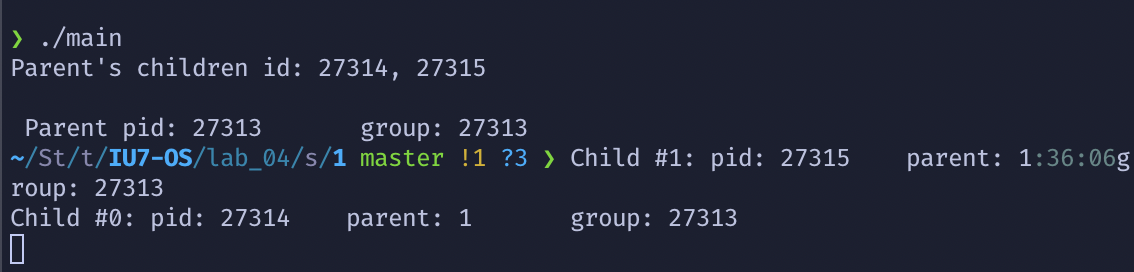
\includegraphics[scale=0.7]{1.png}
	\caption{Демонстрация работы программы (задание №1)}
	\label{fig:1}
\end{figure}

\clearpage
\section*{Задание 2}

Предок ждет завершения своих потомком, используя системный вызов wait(). Вывод соответствующих сообщений на экран. В программе необходимо, чтобы предок выполнял анализ кодов завершения потомков.

\begin{lstlisting}[style=C, caption=Системный вызов wait().]
#include <stdio.h>
#include <unistd.h>
#include <stdlib.h>

int main(void) {
	pid_t ch1, ch2;
	int status;

	ch1 = fork();

	if (ch1 == -1) {
		perror("Can't fork process 0");
		exit(EXIT_FAILURE);
	} else if (ch1 == 0) {
		sleep(2);
		printf("Child #%d: pid: %d\tparent: %d\tgroup: %d\n", 0, getpid(), getppid(), getpgrp());
		exit(EXIT_SUCCESS);
	}

	ch2 = fork();

	if (ch2 == -1) {
		perror("Can't fork process 1");
		exit(EXIT_FAILURE);
	} else if (ch2 == 0) {
		sleep(2);
		printf("Child #%d: pid: %d\tparent: %d\tgroup: %d\n", 1, getpid(), getppid(), getpgrp());
		exit(EXIT_SUCCESS);
	}

	wait(&status);
	
	if (WIFEXITED(status)) {
		puts("\tProcess completed successfully.");
		printf("\tReturn code: %d\n", WEXITSTATUS(status));
	} else if (WIFSIGNALED(status)) {
		puts("\tProcess terminated due to unhandled signal");
		printf("\tSignal number: %d\n", WTERMSIG(status));
	} else if (WIFSTOPPED(status)) {
		puts("\tProcess has been stopped");
		printf("\tSignal number: %d\n", WTERMSIG(status));
	}

	wait(&status);
	
	if (WIFEXITED(status)) {
		puts("\tProcess completed successfully.");
		printf("\tReturn code: %d\n", WEXITSTATUS(status));
	} else if (WIFSIGNALED(status)) {
		puts("\tProcess terminated due to unhandled signal");
		printf("\tSignal number: %d\n", WTERMSIG(status));
	} else if (WIFSTOPPED(status)) {
		puts("\tProcess has been stopped");
		printf("\tSignal number: %d\n", WTERMSIG(status));
	}

	printf("Parent's children id: %d, %d\n", ch1, ch2);

	printf("\n Parent pid: %d\t group: %d\n", getpid(), getpgrp());

	return 0;
}
	
\end{lstlisting}


\begin{figure}[ht]
	\centering
	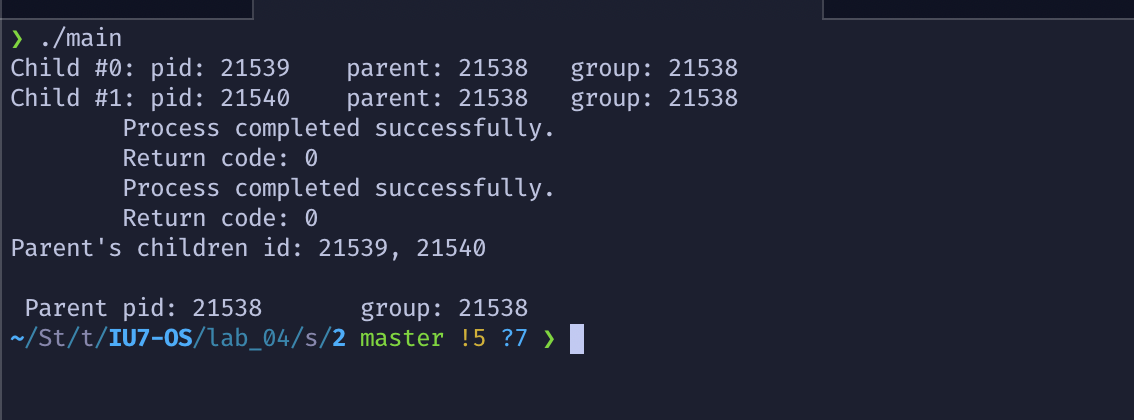
\includegraphics[scale=0.7]{2.png}
	\caption{Демонстрация работы программы (задание №2)}
	\label{fig:2}
\end{figure}

\clearpage
\section*{Задание 3}

Потомки переходят на выполнение других программ. Предок ждет завершения своих потомков. Вывод соответствующих сообщений на экран.

\begin{lstlisting}[style=C, caption=Системный вызов exec().]
#include <stdio.h>
#include <unistd.h>
#include <stdlib.h>

int main(void) {
	pid_t ch1, ch2;
	int status;

	ch1 = fork();

	if (ch1 == -1) {
		perror("Can't fork process 0");
		exit(EXIT_FAILURE);
	} else if (ch1 == 0) {
		printf("Child #%d: pid: %d\tparent: %d\tgroup: %d\n", 0, getpid(), getppid(), getpgrp());

		if (execlp("../../assets/lab_01", "../../assets/lab_01", NULL) == -1) {
			perror("Can't exec child 1\n");
			exit(EXIT_FAILURE);
		}
		exit(EXIT_SUCCESS);
	}

	ch2 = fork();

	if (ch2 == -1) {
		perror("Can't fork process 1");
		exit(EXIT_FAILURE);
	} else if (ch2 == 0) {
		printf("Child #%d: pid: %d\tparent: %d\tgroup: %d\n", 1, getpid(), getppid(), getpgrp());
		
		if (execlp("../../assets/lab_02", "../../assets/lab_02", NULL) == -1) {
			perror("Can't exec child 2\n");
			exit(EXIT_FAILURE);
		}
		exit(EXIT_SUCCESS);
	}

	wait(&status);
	
	if (WIFEXITED(status)) {
		puts("\tProcess completed successfully.");
		printf("\tReturn code: %d\n", WEXITSTATUS(status));
	} else if (WIFSIGNALED(status)) {
		puts("\tProcess terminated due to unhandled signal");
		printf("\tSignal number: %d\n", WTERMSIG(status));
	} else if (WIFSTOPPED(status)) {
		puts("\tProcess has been stopped");
		printf("\tSignal number: %d\n", WTERMSIG(status));
	}

	wait(&status);
	
	if (WIFEXITED(status)) {
		puts("\tProcess completed successfully.");
		printf("\tReturn code: %d\n", WEXITSTATUS(status));
	} else if (WIFSIGNALED(status)) {
		puts("\tProcess terminated due to unhandled signal");
		printf("\tSignal number: %d\n", WTERMSIG(status));
	} else if (WIFSTOPPED(status)) {
		puts("\tProcess has been stopped");
		printf("\tSignal number: %d\n", WTERMSIG(status));
	}

	printf("Parent's children id: %d, %d\n", ch1, ch2);

	printf("\n Parent pid: %d\t group: %d\n", getpid(), getpgrp());

	return 0;
}
		
\end{lstlisting}

\begin{figure}[ht]
	\centering
	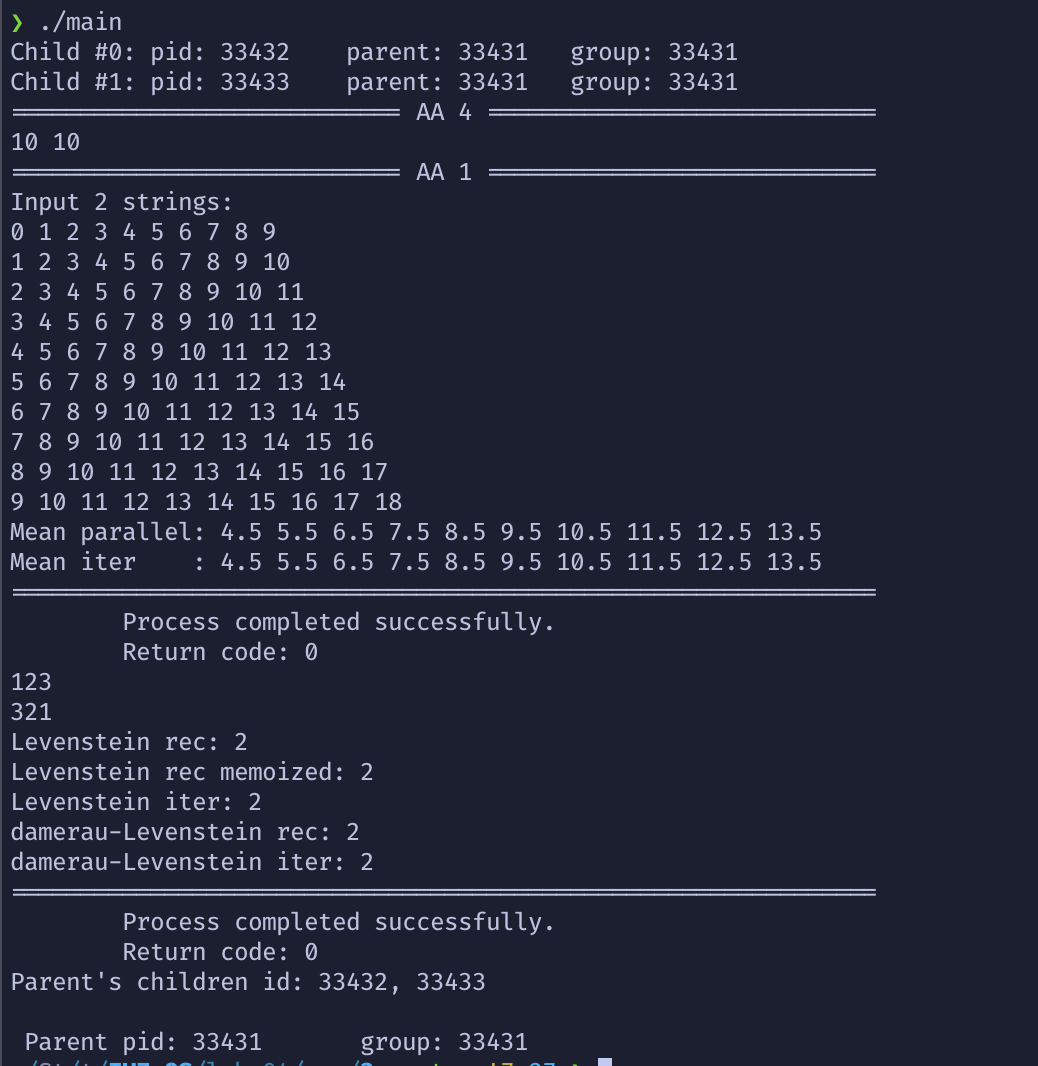
\includegraphics[scale=0.8]{3.png}
	\caption{Демонстрация работы программы (задание №3)}
	\label{fig:3}
\end{figure}

\clearpage
\section*{Задание 4}

Предок и потомки обмениваются сообщениями через неименованный программный канал. Причем оба потомка пишут свои сообщения в один программный канал, а предок их считывает из канала. Потомки должны посылать предку разные сообщения по содержанию и размеру. Предок считывает сообщения от потомков и выводит их на экран. Предок ждет завершения своих потомков и анализирует код их завершения. Вывод соответствующих сообщений на экран.

\begin{lstlisting}[style=C, caption=Системный вызов pipe().]
#include <stdio.h>
#include <unistd.h>
#include <stdlib.h>
#include <string.h>

#include <stdio.h>
#include <unistd.h>
#include <stdlib.h>

const char *msgs[] = { "I like to read books ", "My name is Kirill" };

int main(void) {
	pid_t ch1, ch2;
	int status;

	int fd[2];
	if (pipe(fd) == -1) {
		perror("Cant pipe.");
		return EXIT_FAILURE;
	}

	ch1 = fork();

	if (ch1 == -1) {
		perror("Can't fork process 0");
		exit(EXIT_FAILURE);
	} else if (ch1 == 0) {
		close(fd[0]);
		write(fd[1], msgs[0], strlen(msgs[0]));
		printf("Child #%d: pid: %d\tparent: %d\tgroup: %d\n", 0, getpid(), getppid(), getpgrp());
		exit(EXIT_SUCCESS);
	}

	ch2 = fork();

	if (ch2 == -1) {
		perror("Can't fork process 1");
		exit(EXIT_FAILURE);
	} else if (ch2 == 0) {
		close(fd[0]);
		write(fd[1], msgs[1], strlen(msgs[1]));
		printf("Child #%d: pid: %d\tparent: %d\tgroup: %d\n", 1, getpid(), getppid(), getpgrp());
		exit(EXIT_SUCCESS);
	}

	wait(&status);
	
	if (WIFEXITED(status)) {
		puts("\tProcess completed successfully.");
		printf("\tReturn code: %d\n", WEXITSTATUS(status));
	} else if (WIFSIGNALED(status)) {
		puts("\tProcess terminated due to unhandled signal");
		printf("\tSignal number: %d\n", WTERMSIG(status));
	} else if (WIFSTOPPED(status)) {
		puts("\tProcess has been stopped");
		printf("\tSignal number: %d\n", WTERMSIG(status));
	}

	wait(&status);
	
	if (WIFEXITED(status)) {
		puts("\tProcess completed successfully.");
		printf("\tReturn code: %d\n", WEXITSTATUS(status));
	} else if (WIFSIGNALED(status)) {
		puts("\tProcess terminated due to unhandled signal");
		printf("\tSignal number: %d\n", WTERMSIG(status));
	} else if (WIFSTOPPED(status)) {
		puts("\tProcess has been stopped");
		printf("\tSignal number: %d\n", WTERMSIG(status));
	}

	close(fd[1]);

	const int buff_size = 50;
	char buff[buff_size];

	read(fd[0], buff, buff_size);

	printf("  Read: %s\n", buff);

	printf("Parent's children id: %d, %d\n", ch1, ch2);

	printf("\n Parent pid: %d\t group: %d\n", getpid(), getpgrp());

	return 0;
}
		
\end{lstlisting}

\begin{figure}[ht]
	\centering
	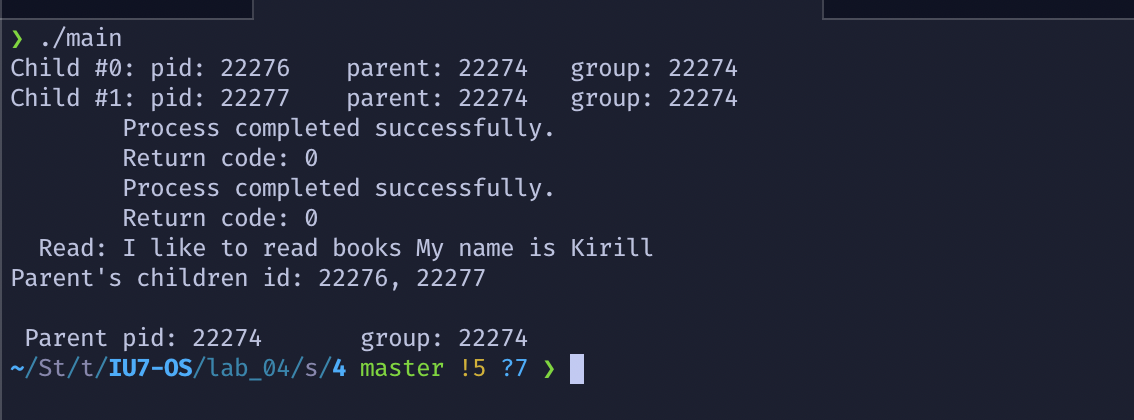
\includegraphics[scale=0.7]{4.png}
	\caption{Демонстрация работы программы (задание №4)}
	\label{fig:4}
\end{figure}

\clearpage
\section*{Задание 5}

Предок и потомки аналогично п.4 обмениваются сообщениями через неименованный программный канал. В программу включается собственный обработчик сигнала. С помощью сигнала меняется ход выполнения программы. При получении сигнала потомки записывают сообщения в канал, если сигнал не поступает, то не записывают. Предок ждет завершения своих потомков и анализирует коды их завершений. Вывод соответствующих сообщений на экран.

\begin{lstlisting}[style=C, caption=Системный вызов signal().]
#include <stdio.h>
#include <unistd.h>
#include <stdlib.h>
#include <string.h>

const char *msgs[] = { "I like to read books ", "My name is Kirill" };
int state = 0;

void dummy(int snum) {}

void sig_catcher(int snum)
{
	state = 1;
}

int main(void)
{
	pid_t ch1, ch2;
	int status;

	int fd[2];
	if (pipe(fd) == -1)
	{
		perror("Cant pipe.");
		return EXIT_FAILURE;
	}

	signal(SIGINT, dummy);

	ch1 = fork();

	if (ch1 == -1)
	{
		perror("Can't fork process 0");
		exit(EXIT_FAILURE);
	}
	else if (ch1 == 0)
	{
		signal(SIGINT, sig_catcher);
		sleep(3);
		if (state)
		{
			close(fd[0]);
			write(fd[1], msgs[0], strlen(msgs[0]));
			puts("Message has been sent");
		}
		else
		{
			puts("No signal has been caught.");
		}
		printf("Child #%d: pid: %d\tparent: %d\tgroup: %d\n", 0, getpid(), getppid(), getpgrp());
		exit(EXIT_SUCCESS);
	}

	ch2 = fork();

	if (ch2 == -1)
	{
		perror("Can't fork process 1");
		exit(EXIT_FAILURE);
	}
	else if (ch2 == 0)
	{
		signal(SIGINT, sig_catcher);
		sleep(3);
		if (state)
		{
			close(fd[0]);
			write(fd[1], msgs[1], strlen(msgs[1]));
			puts("Message has been sent");
		}
		else
		{
			puts("No signal has been caught.");
		}
		printf("Child #%d: pid: %d\tparent: %d\tgroup: %d\n", 1, getpid(), getppid(), getpgrp());
		exit(EXIT_SUCCESS);
	}

	wait(&status);
	
	if (WIFEXITED(status)) {
		puts("\tProcess completed successfully.");
		printf("\tReturn code: %d\n", WEXITSTATUS(status));
	} else if (WIFSIGNALED(status)) {
		puts("\tProcess terminated due to unhandled signal");
		printf("\tSignal number: %d\n", WTERMSIG(status));
	} else if (WIFSTOPPED(status)) {
		puts("\tProcess has been stopped");
		printf("\tSignal number: %d\n", WTERMSIG(status));
	}

	wait(&status);
	
	if (WIFEXITED(status)) {
		puts("\tProcess completed successfully.");
		printf("\tReturn code: %d\n", WEXITSTATUS(status));
	} else if (WIFSIGNALED(status)) {
		puts("\tProcess terminated due to unhandled signal");
		printf("\tSignal number: %d\n", WTERMSIG(status));
	} else if (WIFSTOPPED(status)) {
		puts("\tProcess has been stopped");
		printf("\tSignal number: %d\n", WTERMSIG(status));
	}

	close(fd[1]);

	const int buff_size = 50;
	char buff[buff_size];

	read(fd[0], buff, buff_size);

	printf("  Read: %s\n", buff);

	printf("Parent's children id: %d, %d\n", ch1, ch2);

	printf("\n Parent pid: %d\t group: %d\n", getpid(), getpgrp());

	return 0;
}
\end{lstlisting}

\begin{figure}[ht]
	\centering
	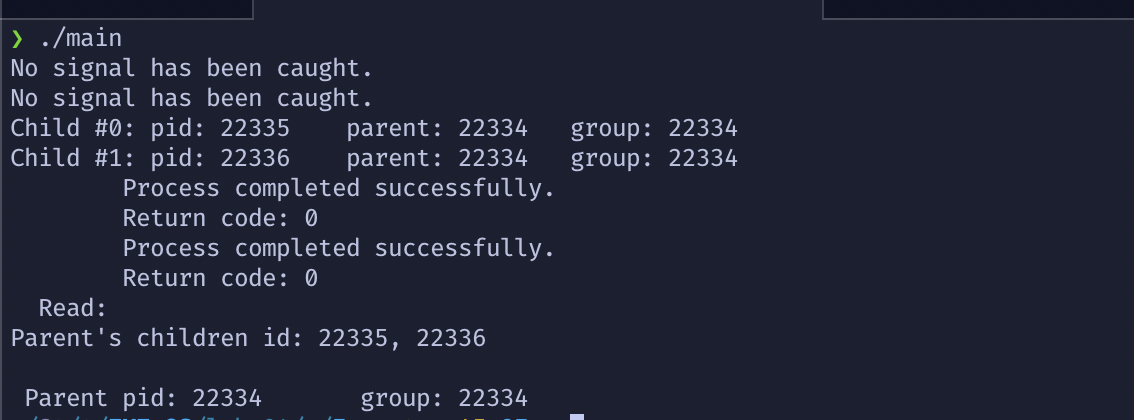
\includegraphics[scale=0.7]{5_1.png}
	\caption{Демонстрация работы программы, сигнал не вызывается (задание №5)}
	\label{fig:5_1}
\end{figure}

\begin{figure}[ht]
	\centering
	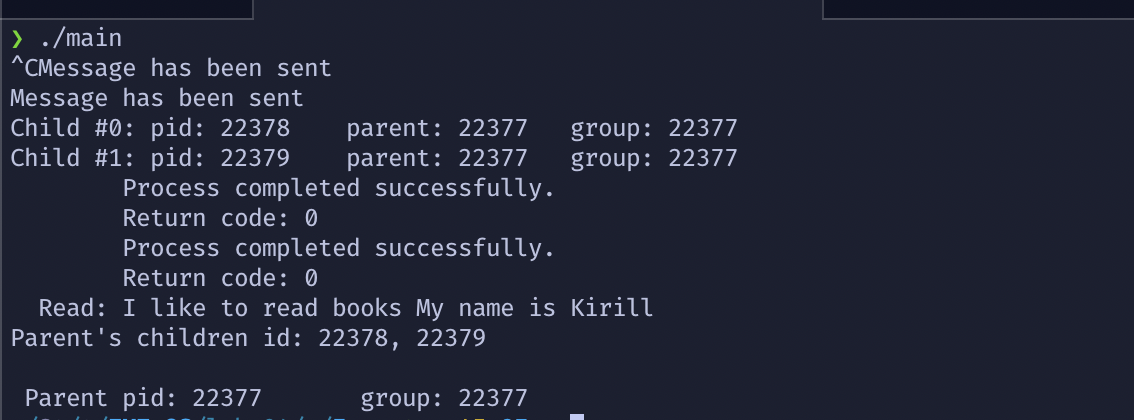
\includegraphics[scale=0.7]{5_2.png}
	\caption{Демонстрация работы программы, сигнал вызывается (задание №5)}
	\label{fig:5_2}
\end{figure}

\begin{figure}[ht]
	\centering
	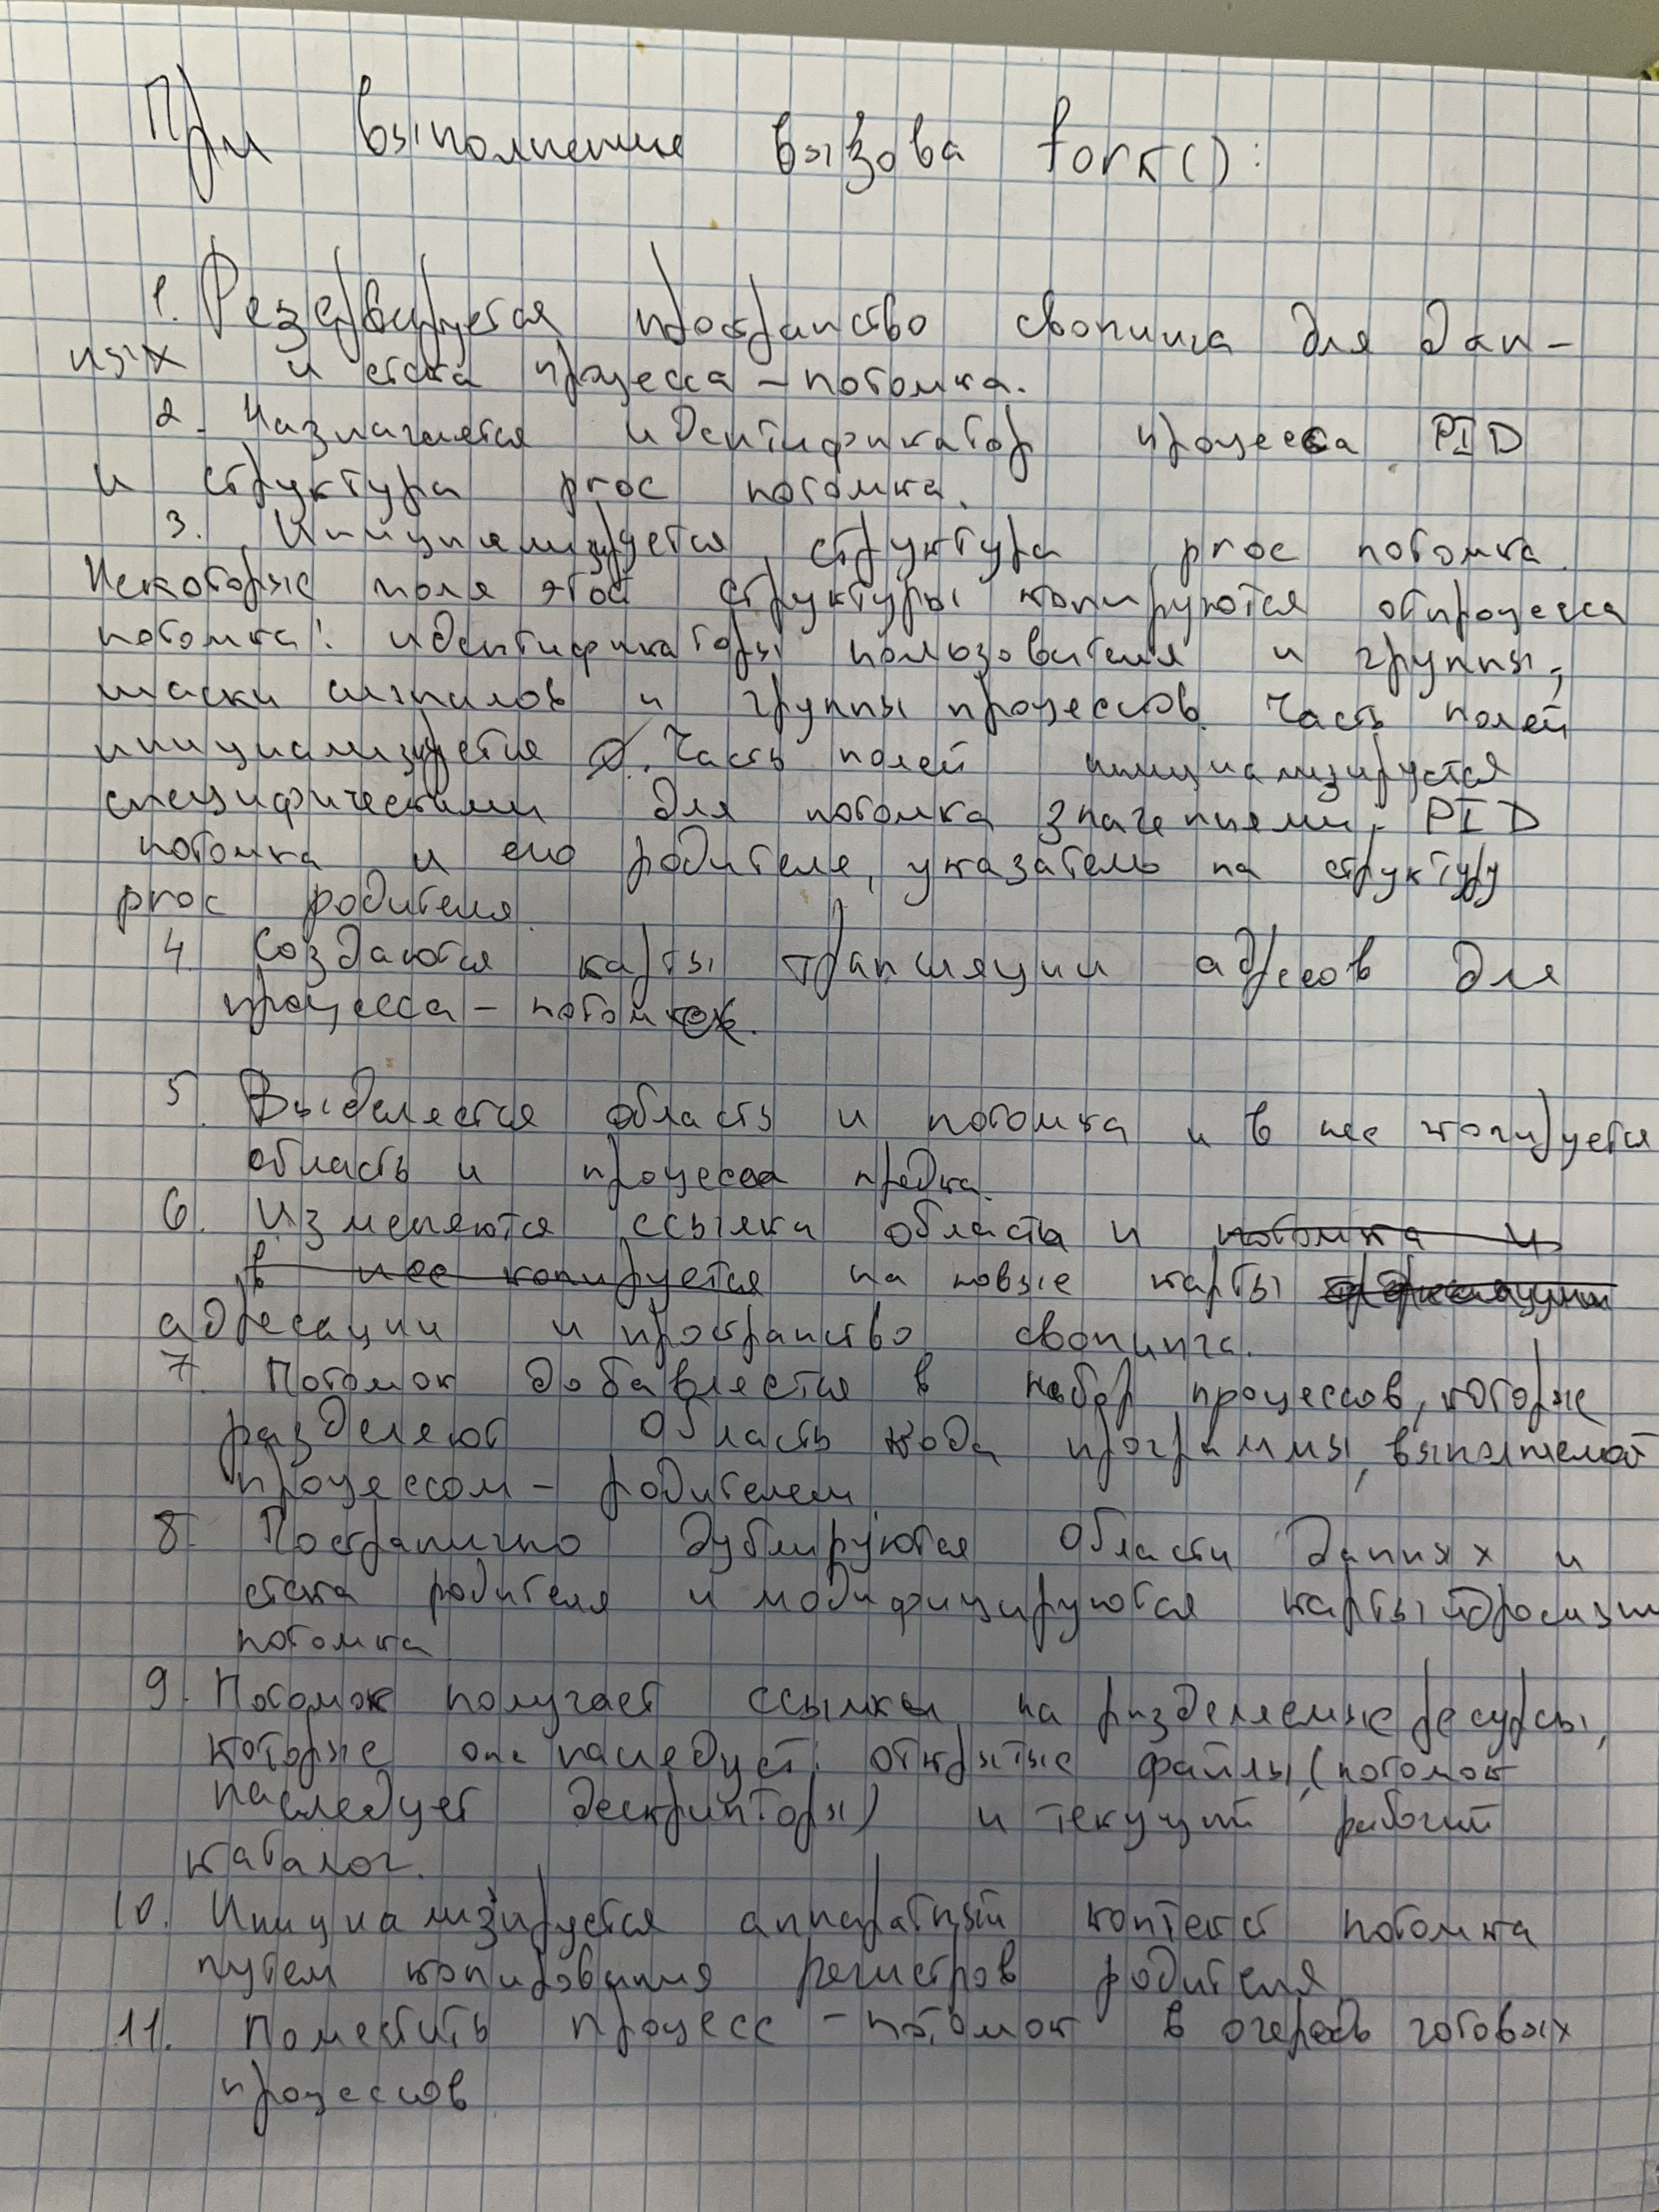
\includegraphics[scale=0.15]{6.jpeg}
	\caption{Очередность при вызове fork()}
	\label{fig:6}
\end{figure}

\begin{figure}[ht]
	\centering
	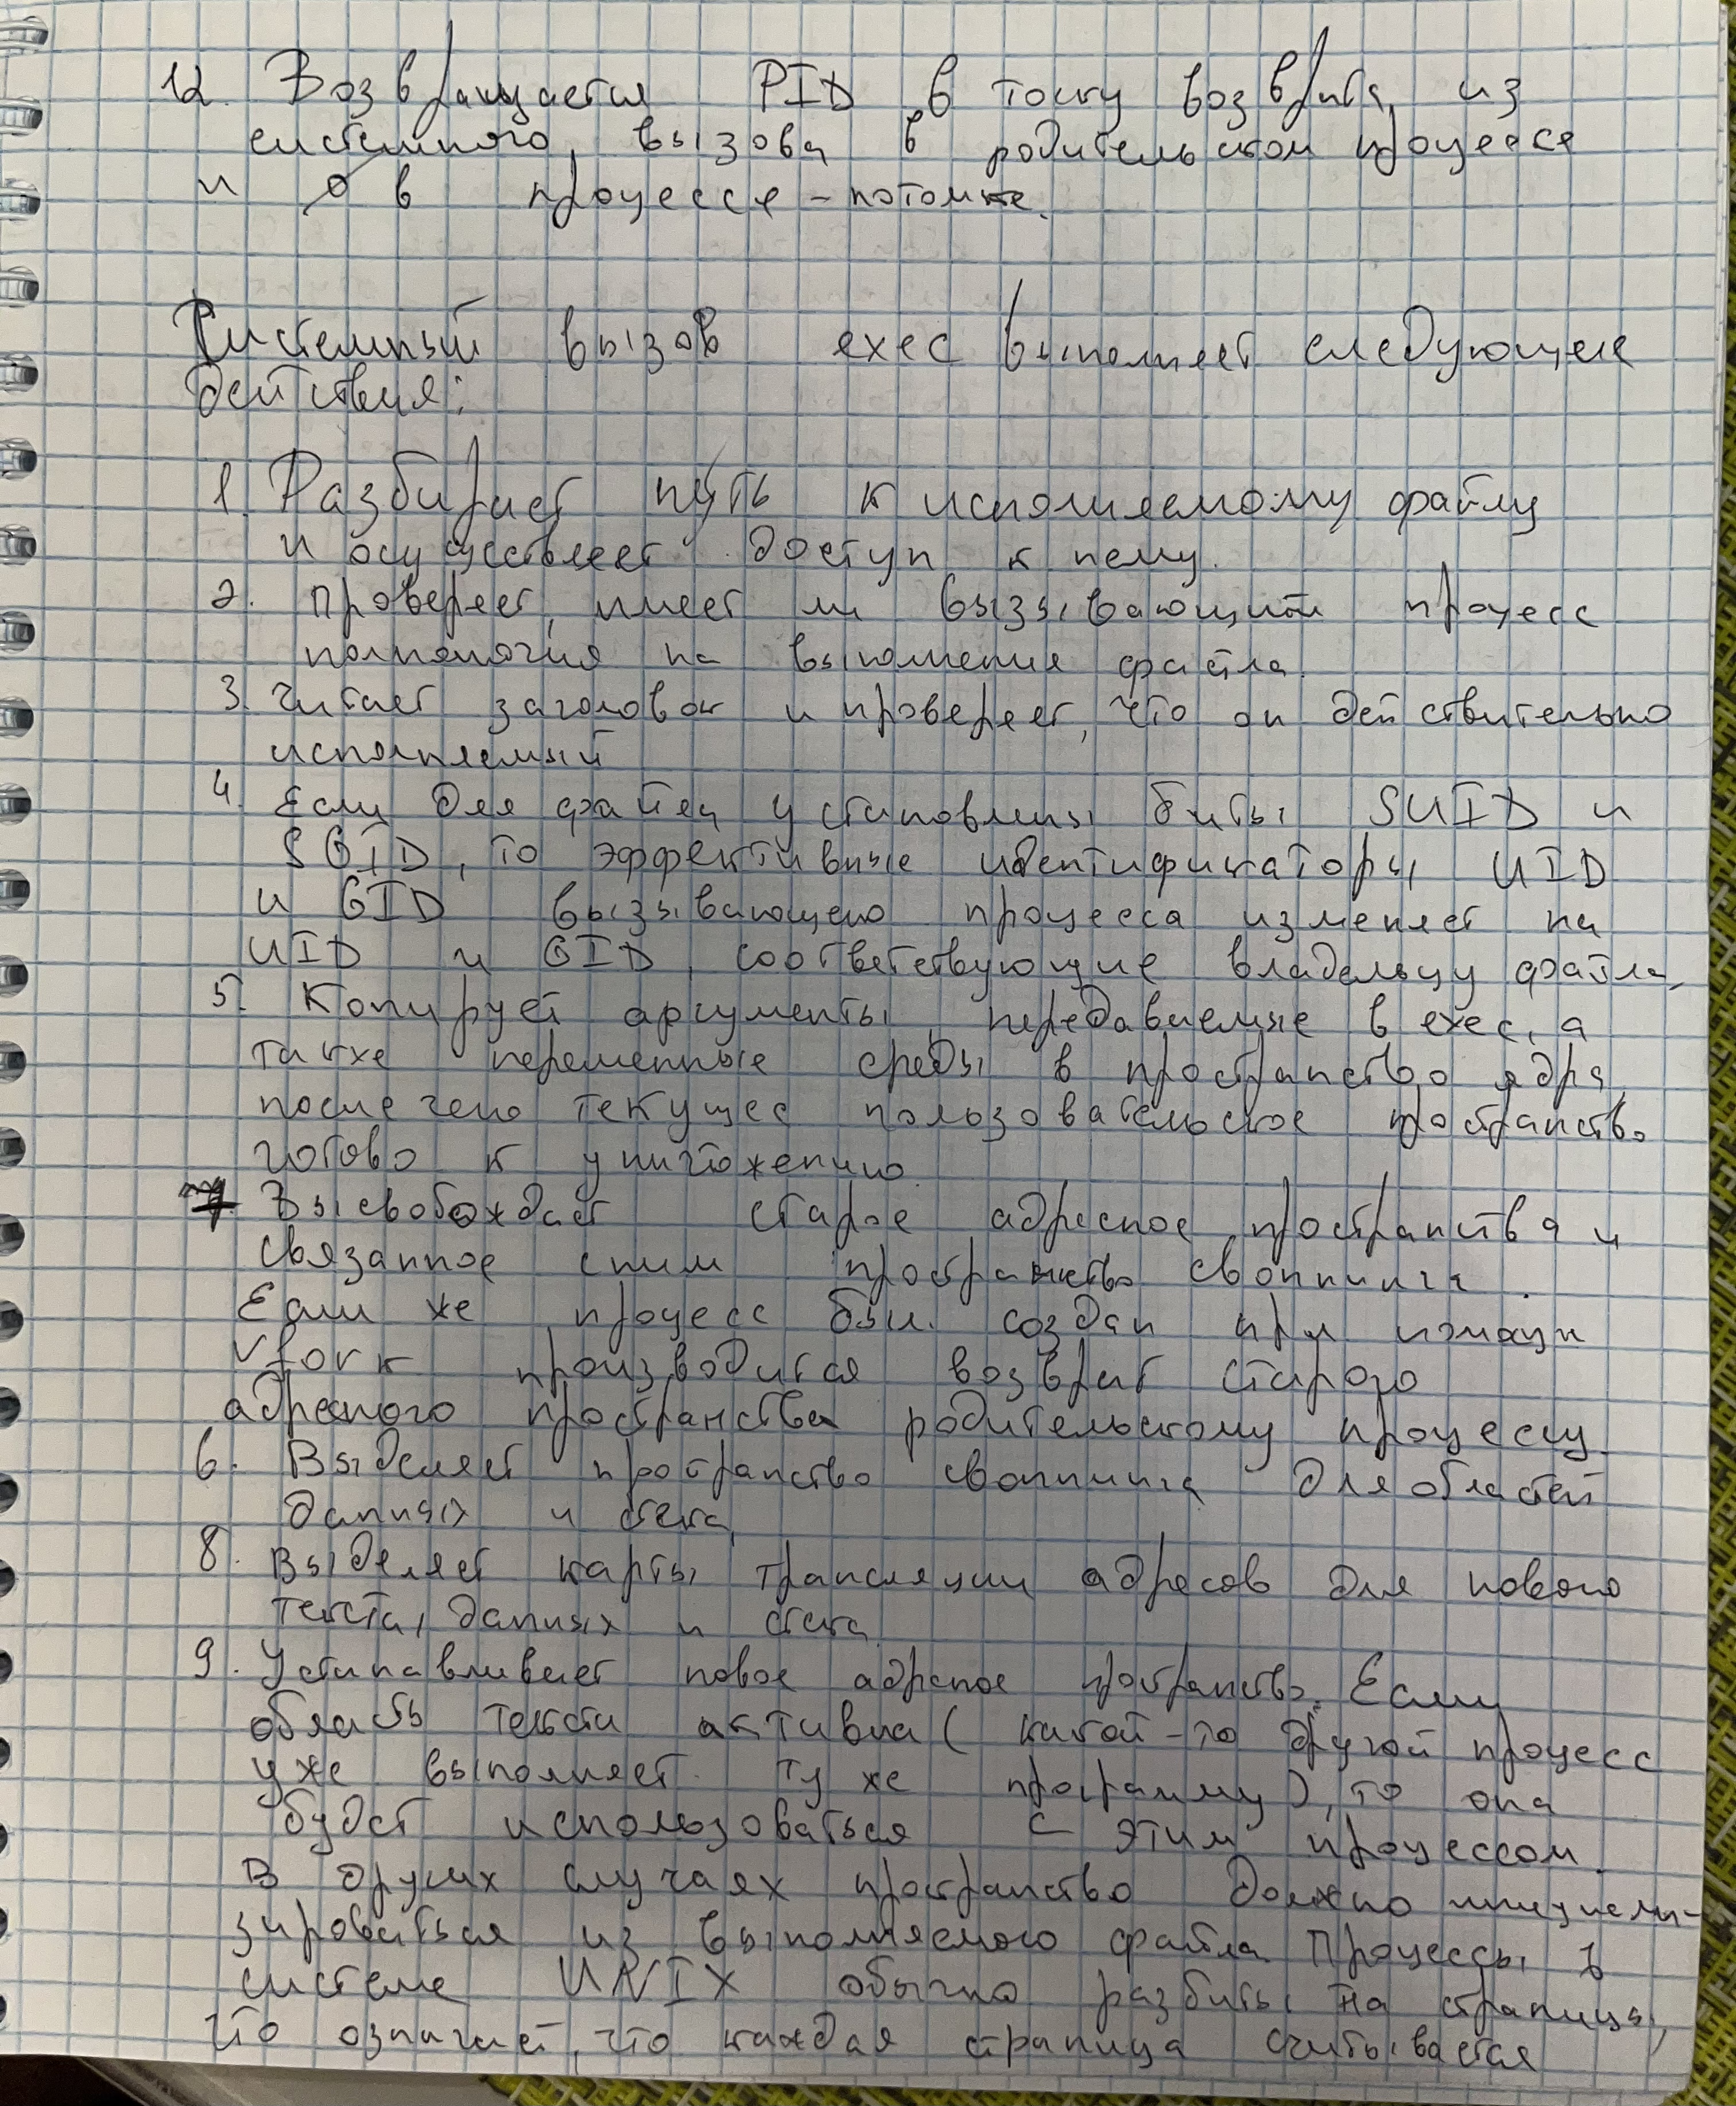
\includegraphics[scale=0.15]{7.jpeg}
	\caption{Очередность при вызове fork()}
	\label{fig:7}
\end{figure}

\begin{figure}[ht]
	\centering
	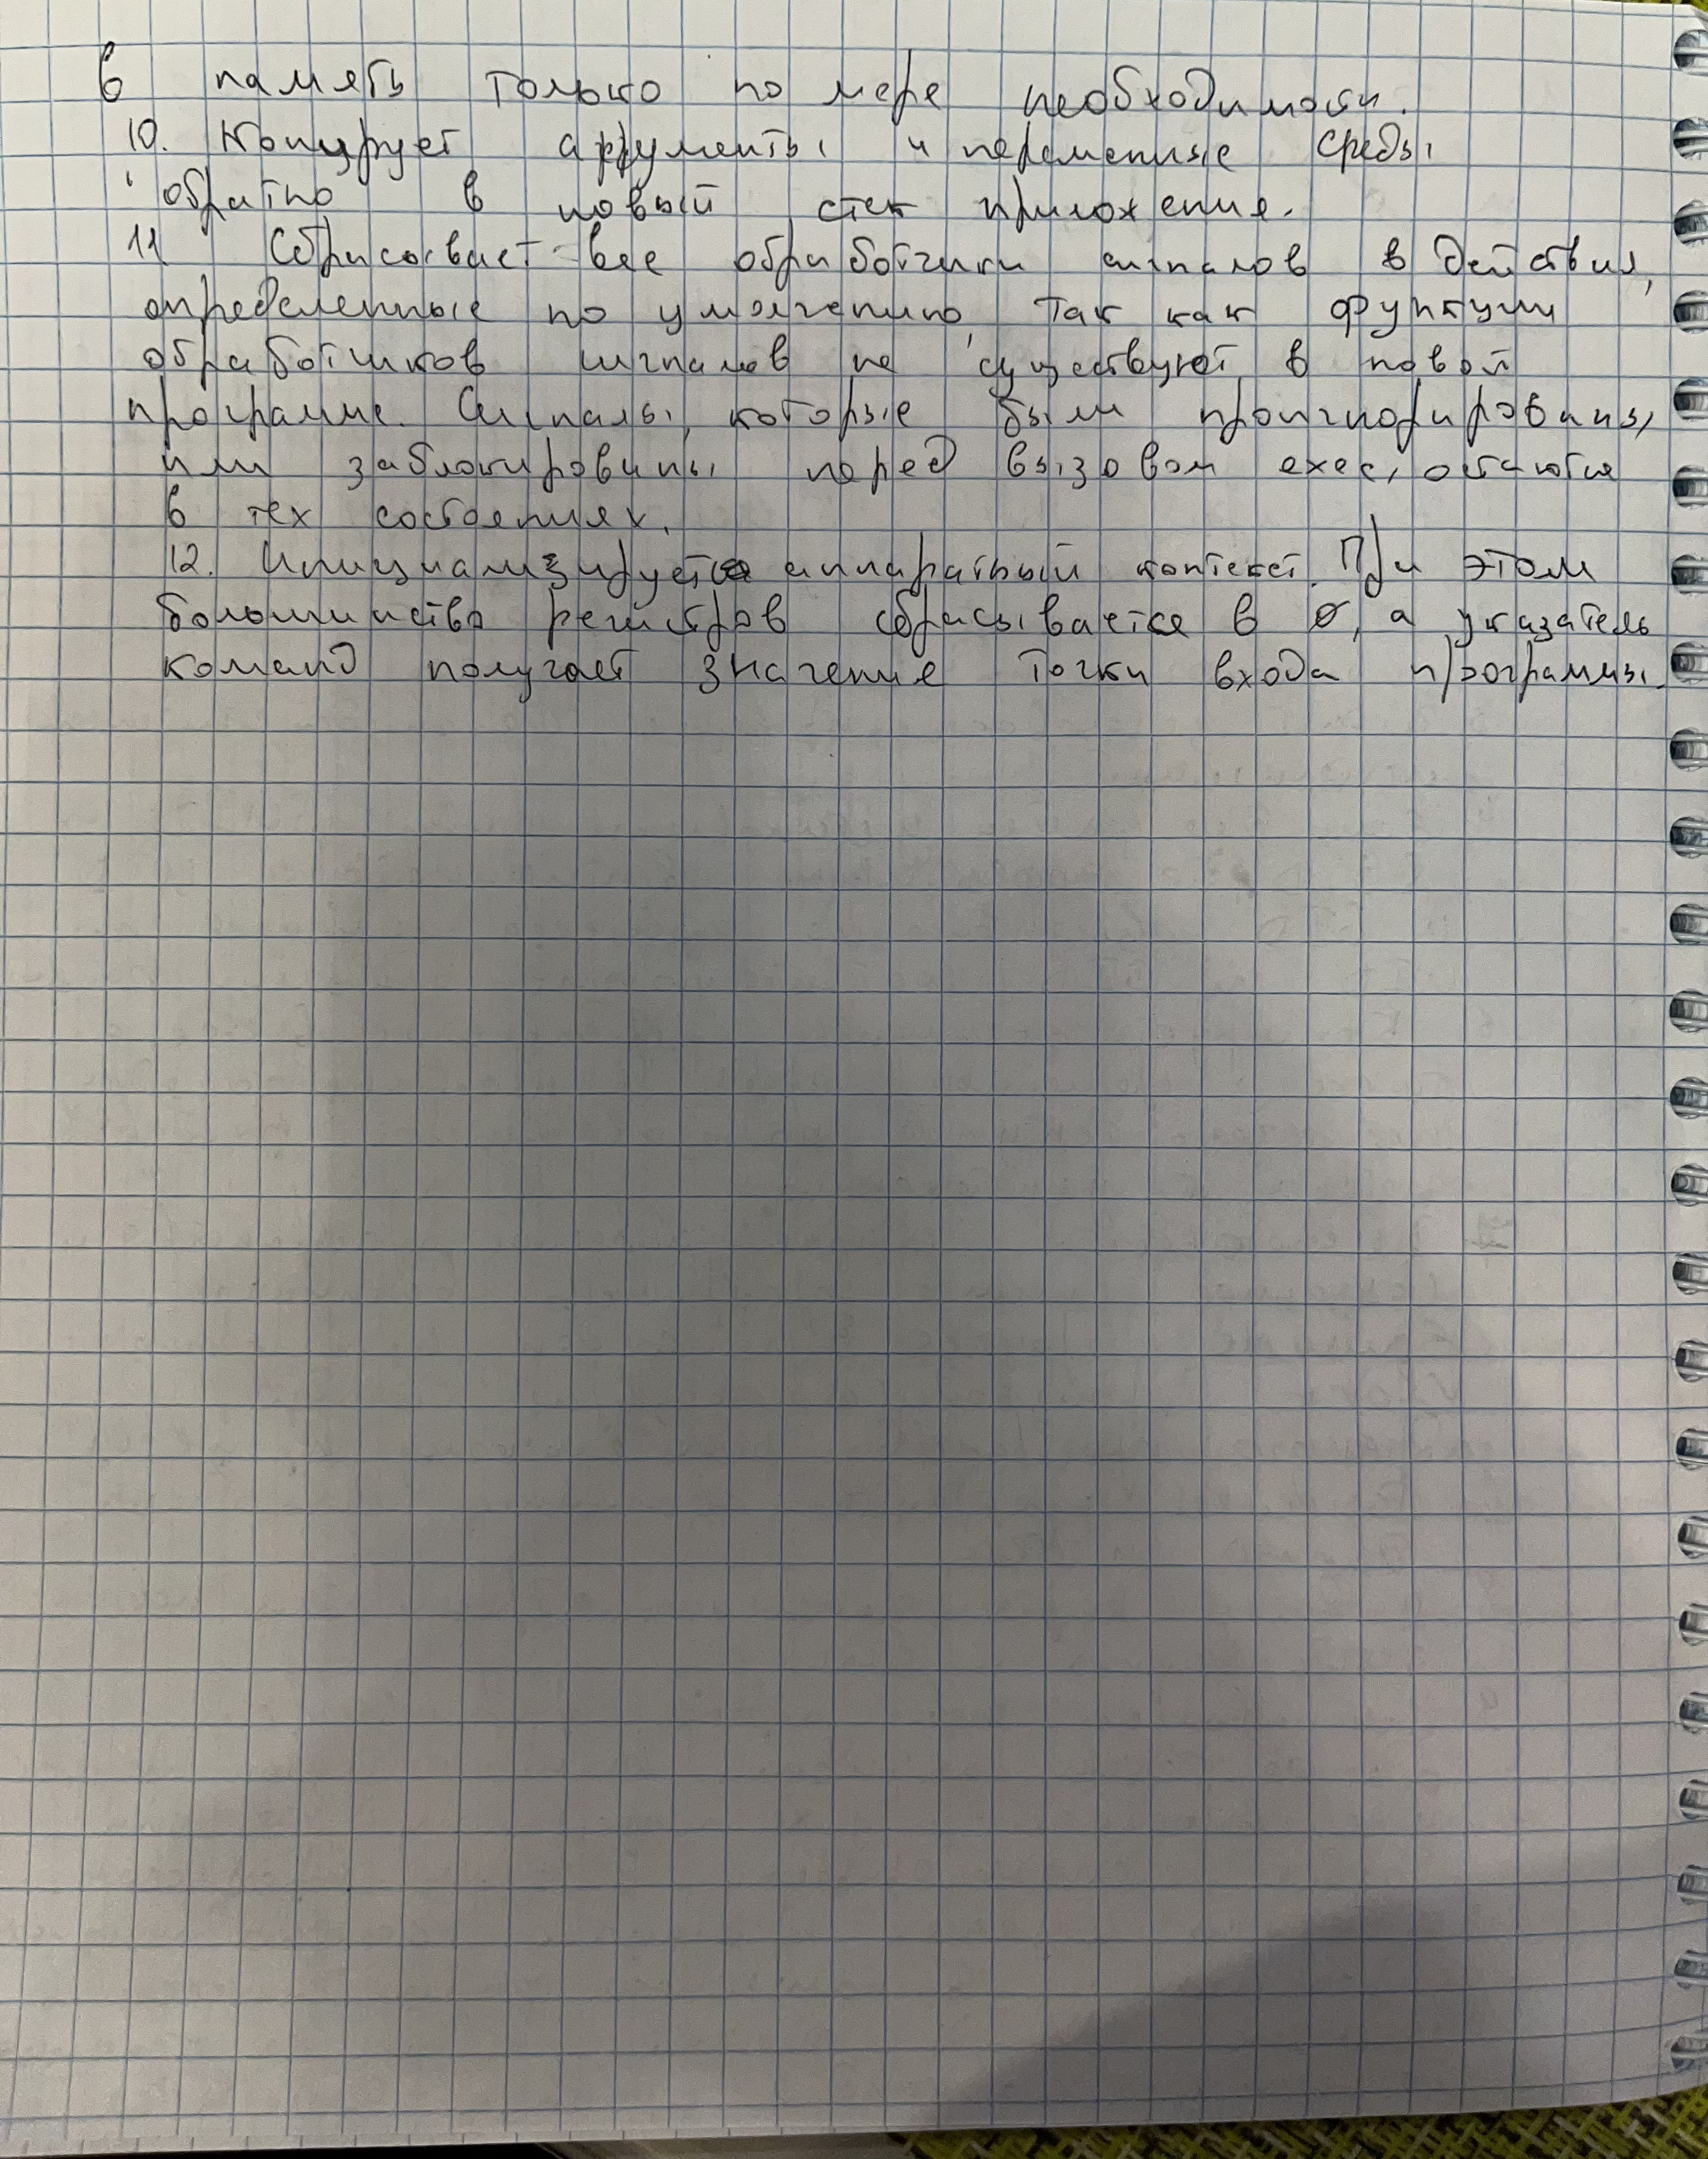
\includegraphics[scale=0.15]{8.jpeg}
	\caption{Очередность при вызове exec()}
	\label{fig:8}
\end{figure}

\end{document}
